\part{Rendu}
    Après avoir détecté le tag dans l'image, la seconde grande étape est de projeter un modèle 3D sur la scène. Pour cela, l'utilisateur indique au lancement du programme le ou les modèles à utiliser, avec ou non des matériaux, et ceux-ci seront rendus à chaque image. Toujours dans le principe du "from scratch", nous avons décidé de ne pas utiliser de moteur de rendu déjà fonctionnel tel qu'OpenGL, mais de redévelopper le nôtre.

    \section{Gestion des objets}

        \subsection{Objets}

            \subsubsection{Définition du format}                
                Un objet 3D est composé de sommets, formant des faces d'au moins 3 côtés. Le format le plus simple pour stocker un modèle 3D est le \emph{.obj}. Cette norme définit les sommets, les matériaux et les normales pour chaque face dans un format texte. Chaque ligne débute par un indicateur puis les valeurs à proprement parler. Un exemple est visible figure \ref{fig:obj}. Nous utilisons 4 indicateurs :
                \begin{itemize}
                    \item v x y z : sommet à la position $(x, y, z)$
                    \item vt u v [w] : coordonnées de texture (voir partie \ref{subsubsec:materiaux})
                    \item vn x y z : normale (voir partie \ref{subsubsec:lumiere})
                    \item f v/vt/vn [...] : les faces de l'objet avec un triplet d'indice pour chaque sommet (minimum 3). La coordonnée de texture peut être vide (v//vn).
                \end{itemize}
                
                \begin{figure}[h]
                    \centering
                    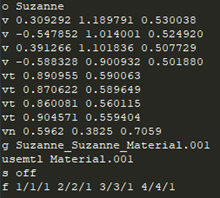
\includegraphics[scale=0.8]{img/rendu/obj.png}
                    \caption{Exemple de fichier \emph{.obj}}
                    \label{fig:obj}
                \end{figure}
                Nous avons écrit un parser afin de décomposer ce fichier \emph{.obj}.

                Chaque objet est contenu dans une classe \emph{Object}. Celle-ci contient un ensemble de faces qui correspond à plusieurs points, une couleur et une normale. Plusieurs fonctions sont également disponibles afin de manipuler l'objet : \emph{rotate}, \emph{scale}, \emph{position}\dots

            \subsubsection{Matériaux}
            \label{subsubsec:materiaux}

            Afin de rendre les objets plus agréables à l'\oe il, nous avons décidé d'implémenter la gestion des matériaux. Nous utilisions déjà le format \emph{.obj} pour les modèles, il semblait donc naturel d'utiliser les \emph{.mtl}, format défini par la même norme, pour les matériaux. 

            Un fichier \emph{.mtl} est un fichier texte, et nous utilisons uniquement une seule ligne de ce fichier, \emph{map\_kD}, qui indique le nom de l'image texture utilisée. Les coordonnées de texture renseignées dans le \emph{.obj} indiquent des pourcentages dans cette image, respectivement $u$, $v$, la largeur et la hauteur. Nous travaillons ici avec des images 2D.

            \begin{figure}[h]
                \centering
                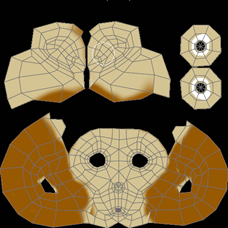
\includegraphics[scale=0.8]{img/rendu/texture.png}
                \caption{Texture découpée par face}
                \label{fig:texture}
            \end{figure}

            Dans la figure \ref{fig:texture}, nous pouvons voir les faces en fonction des coordonnées indiquées pour chaque sommet. Afin de pouvoir utiliser cette texture, il faut déformer le polygone (en utilisant une homographie) pour l'appliquer sur le polygone projeté. Cependant, cette étape est très coûteuse en performance, car il faut l'appliquer à chaque polygone de chaque objet à chaque image de la vidéo. Nous avons alors choisi de préférer le temps réel et, pour cela, une face ne possède qu'une seule couleur, inscrite directement dans la classe \emph{Object}. Pour choisir la couleur, nous prenons simplement la couleur du pixel au centre du polygone sur l'image texture. Cela nous donne alors un objet avec des couleurs unies pour les faces. 
            
            Une amélioration possible du programme pourrait être de prendre en compte les autres paramètres du fichier \emph{.mtl} et donc de ne pas obligatoirement utiliser d'image pour la texture.

        \subsection{Scène}

            La scène est un regroupement de tous les objets et de la caméra. Afin de donner une liberté à l'utilisateur et de ne pas recompiler à chaque fois le programme, nous avons défini un format CSV \emph{.scene} (figure \ref{fig:scene}) qui défini chaque objet de la scène ainsi que leur position et leur rotation.

            \begin{figure}[h]
                \centering
                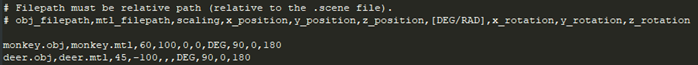
\includegraphics[scale=0.8]{img/rendu/scene.png}
                \caption{Fichier CSV \emph{.scene}}
                \label{fig:scene}
            \end{figure}

            Chaque champ est optionnel, à l'exception du premier qui définit l'objet à charger. Un champ vide prendra une valeur par défaut inscrite dans le code.

            Notre méthode pour le placement et l'échelle des objets à cependant un défaut. Il faut déterminer à la main la bonne position et la bonne échelle pour que l'objet soit visible et au bon endroit. En effet, deux logiciels de modélisation n'enregistrent pas l'échelle de la même façon. Par exemple, avec Blender, une échelle entre 45 et 55 est idéale. Tous les \emph{.obj} fournis dans le projet ont été créés par nous-mêmes sous Blender.

        \subsection{Lumière}
        \label{subsubsec:lumiere}

        Une méthode d'ombrage plat (\textit{Flat Shading}) a été implémentée afin de rendre l'apparence des objets plus réaliste. La lumière est représentée par un vecteur qui donne sa direction. Afin de déterminer l'éclairage d'une face, nous utilisons la normale définie dans le \emph{.obj}. Nous ne souhaitons qu'une seule illumination par face, nous calculons alors la moyenne des normales des sommets que nous enregistrons dans la face avec la couleur et les points. 

        Ensuite, la luminosité est calculée pour chaque face en fonction de l'angle entre sa normale et la direction de la lumière. Plus l'angle est proche de 0\degree, plus les vecteurs sont alignés et donc plus la face est dans l'ombre. Inversement, plus l'angle est proche de 180\degree, plus la face est éclairée. Cet angle est normalisé puis multiplié à la couleur de la face. Nous pouvons voir cet effet, avec les matériaux, dans la figure \ref{fig:lumiere}. Le rendu sera expliqué dans la partie suivante.

        \begin{figure}[h]
            \centering

            \subfloat[][]{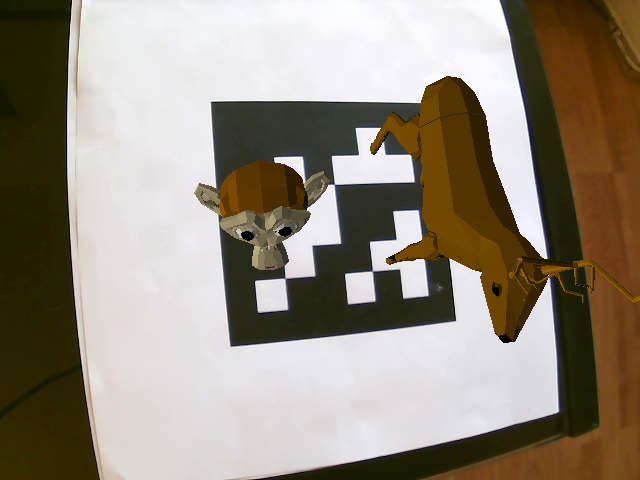
\includegraphics[width=0.49\linewidth]{img/rendu/flat_shading_left.png}}
            \hspace{.005\textwidth}
            \subfloat[][]{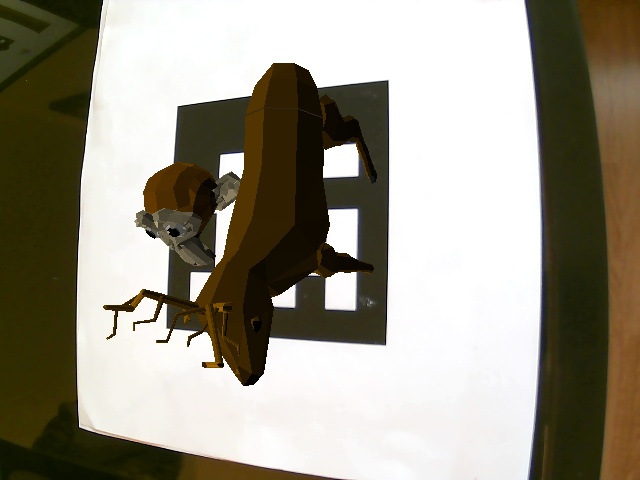
\includegraphics[width=0.49\linewidth]{img/rendu/flat_shading_right.png}}

            \caption{Ombrage plat sur les objets à partir d'une source lumineuse venant de la gauche}
            \label{fig:lumiere}
        \end{figure}

    \section{Caméra et projection}
        Après avoir chargé les objets dans la scène 3D, il faut les projeter sur l'image en fonction du tag. Nous utilisons cette relation :
        \begin{equation*}
            \begin{pmatrix}
                u \\ v \\ 1
            \end{pmatrix}
            = K.E.
            \begin{pmatrix}
                x_w \\ y_w \\ z_w \\ 1
            \end{pmatrix}
        \end{equation*}
        avec $u,v$ les coordonnées dans le plan image en pixels, $K$ les paramètres intrinsèques de la caméra, $E$ les rotations et translation de la caméra dans le repère monde et $x_w, y_w, z_w$ les coordonnées du point 3D dans le repère monde.

        \subsection{Calibration}
            Afin de déterminer les paramètres intrinsèques de la caméra, nous avons développé une fonction pour les calculer. Elle se base sur la prise de photos de checkerboard tel que la figure \ref{fig:checkerboard}.

            \begin{figure}[!h]
                \centering
                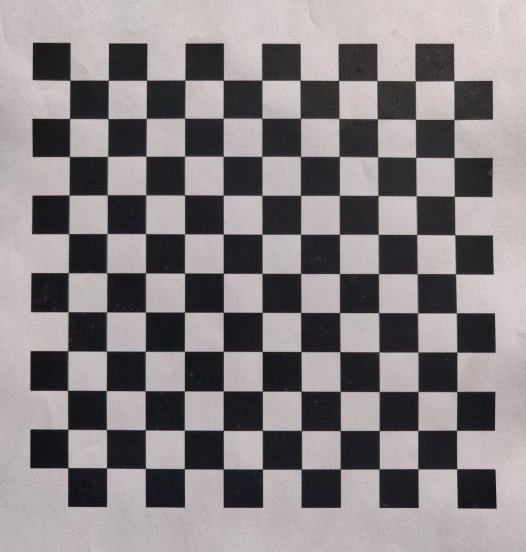
\includegraphics[scale=0.3]{img/rendu/checkerboard.jpg}
                \caption{Exemple de checkerboard}
                \label{fig:checkerboard}
            \end{figure}

            Des images de différents angles sont nécessaires. Après quelques essais, environ 5-6 images sont suffisantes pour estimer les paramètres. La méthode se base principalement sur la fonction \verb|cv::calibrateCamera| d'OpenCV. Elle prend en paramètres les coordonnées des points 3D et leur correspondance sur l'image (les points 2D). Étant donné que le checkerboard est connu, on peut donner des coordonnées à chaque coin des carrés en supposant que $z=0$, ces points étant sur le même plan. Les coins du checkerboard sur l'image peuvent être trouvés par la fonction \verb|cv::findChessboardCorners| d'OpenCV.

            Après avoir calculer les paramètres intrinsèques, nous les enregistrons dans un format texte avec l'extension \emph{.cam} (figure \ref{fig:cam})

            \begin{figure}[!h]
                \centering
                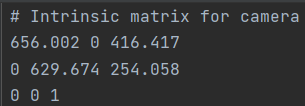
\includegraphics[scale=0.8]{img/rendu/cam.png}
                \caption{Fichier \emph{.cam} représentant les paramètres intrinsèques}
                \label{fig:cam}
            \end{figure}

            Ce fichier se compose d'une matrice 3x3 représentant les paramètres intrinsèques ainsi :
            \begin{equation*}
                \begin{pmatrix}
                    f_x & s & x_0 \\
                    0 & f_y & y_0 \\
                    0 & 0 & 1
                \end{pmatrix}
            \end{equation*}
            $f$ est la distance focale en pixels. Dans une caméra parfaite, $f_x$ et $f_y$ sont égaux mais en pratique, ils peuvent différer, ce qui cause des pixels non carrés. $s$ est une distorsion de l'image, souvent égale à 0, ce qui est suffisant dans notre cas. Enfin $(x_0, y_0)$ est le centre optique de l'image, l'intersection entre l'axe optique et le plan image. Il est en général plus ou moins au centre de l'image. 

        \subsection{Projection}
        \label{subsec:projection}
            Ayant les paramètres intrinsèques de la caméra, nous pouvons maintenant rendre les objets 3D. À chaque frame, nous devons mettre à jour la matrice de projection de la caméra.

            \subsubsection{Matrice de projection}
                La matrice de projection est la multiplication matricielle de $K$ et $E$. Après l'avoir calculé, il suffit donc de la multiplier à un point 3D pour avoir ses coordonnées dans le plan image.

                Afin de mettre à jour la matrice de projection, nous calculons tout d'abord une homographie $H_i$ entre les points du tag et un carré parfait comme défini dans la partie \ref{subsubsec:homographie}. Le calcul de l'homographie est une opération inversible, on peut facilement calculer l'homographie allant du carré parfait aux points du tag en inversant la matrice $H_i$, ce qui nous donne une matrice $H$. L'homographie $H$ contient les mêmes informations que la position la caméra $K.E$ ($E = [R|t]$). Il est nécessaire de la normaliser. 

                On peut donc estimer la position de la caméra ainsi :
                $R^1$ et $R^2$ sont les premières colonnes de $H$. $t$ est la dernière colonne de $H$. Étant donné que les rotations doivent être orthogonales, car on se place dans un repère orthonormé 3D, on peut calculer $R^3$ avec le produit vectoriel de $R^1$ et $R^2$ donc $R^3 = R^1 \times R^2$.

                En résumé nous avons :
                \begin{equation*}
                    E = [R|t] = [H^1 | H^2 | H^1\times H^2 | H^3]
                \end{equation*}
                Nous pouvons donc calculer $K.E$, la matrice de projection.
                
                Chaque point d'une face est alors projeté sur l'image en multipliant $K.E$ par le point. On utilise des coordonnées homogènes, il est donc nécessaire de diviser $u$ et $v$ par la troisième coordonnée afin d'obtenir 1 à cette dernière. 

                Le polygone projeté est alors rempli en utilisant la fonction \verb|cv::fillConvexPoly| avec la couleur de la face multipliée par sa luminosité (voir partie \ref{subsubsec:lumiere}). Nous pouvons voir le résultat de ces opérations dans la figure \ref{fig:sans_peintre}.

                \begin{figure}[!h]
                    \centering
                    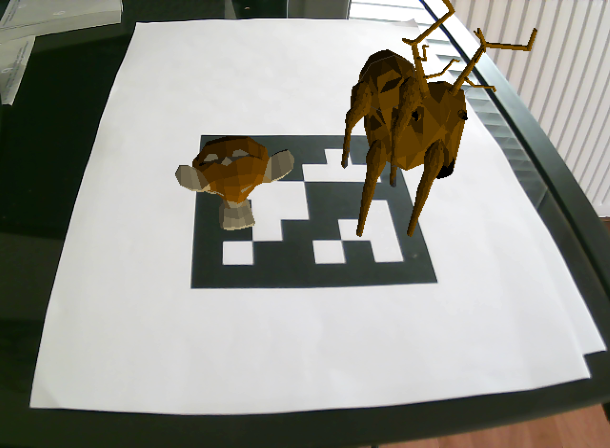
\includegraphics[scale=0.45]{img/rendu/sans_peintre.png}
                    \caption{Rendu d'une scène sans l'algorithme du peintre}
                    \label{fig:sans_peintre}
                \end{figure}
                
            \subsubsection{Algorithme du peintre}
                Nous pouvons tout de suite voir un problème dans la figure \ref{fig:sans_peintre}, les faces arrière sont parfois dessinées sur les faces avant, ce qui rend l'image très confuse. Le moyen le plus simple de le résoudre est l'algorithme du peintre. Il consiste à dessiner les faces les plus loin en premier puis se rapprocher de la caméra petit à petit. Ainsi les polygones les plus proches vont recouvrir les autres. 

                \begin{figure}[!h]
                    \centering
                    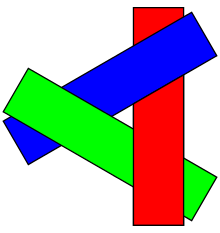
\includegraphics[scale=0.3]{img/rendu/peintre_probleme.png}
                    \caption{Agencement de polygones problématique}
                    \label{fig:peintre_probleme}
                \end{figure}

                Cet algorithme n'est pas parfait et peut ne pas fonctionner dans certains cas d'utilisation précis, comme celui de la figure \ref{fig:peintre_probleme}. Il n'est pas non plus très efficient, car il demande de calculer des faces qui seront cachées par la suite. Cependant, il est suffisant à notre cas et a donc été choisi. 

                Nous extrayons tout d'abord la translation de la caméra de la matrice de projection suivant cette formule : 
                \begin{equation*}
                    E = K^{-1}.K.E = [R|t]
                \end{equation*}
                Grâce à cela, nous pouvons calculer la distance à la caméra d'une face en prenant la norme de la différence du vecteur $t$ et du centre de la face. En utilisant ce calcul, il est possible de trier les faces en fonction de leur distance. Il suffit par la suite de projeter par les faces les plus loin en premier. Nous obtenons donc ainsi un rendu réaliste visible à la figure \ref{fig:avec_peintre}.

                \begin{figure}[!h]
                    \centering
                    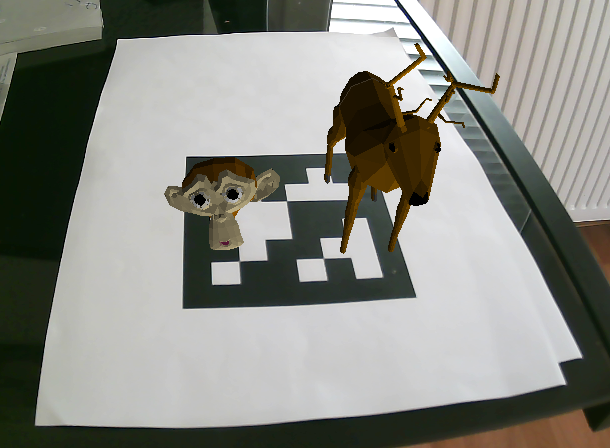
\includegraphics[scale=0.45]{img/rendu/avec_peintre.png}
                    \caption{Rendu d'une scène avec l'algorithme du peintre}
                    \label{fig:avec_peintre}
                \end{figure}

                Les différents objets sont gérés simplement en regroupement toutes les faces de tous les objets avant de les trier pour les projeter. 
